\documentclass{beamer}

\usepackage{amssymb,amsmath}
\usepackage{graphicx}
\usepackage{url}
\usepackage{color}
\usepackage{relsize}		% For \smaller
\usepackage{url}			% For \url
\usepackage{epstopdf}	% Included EPS files automatically converted to PDF to include with pdflatex

%For MindMaps
% \usepackage{tikz}%
% \usetikzlibrary{mindmap,trees,arrows}%

%%% Color Definitions %%%%%%%%%%%%%%%%%%%%%%%%%%%%%%%%%%%%%%%%%%%%%%%%%%%%%%%%%
%\definecolor{bordercol}{RGB}{40,40,40}
%\definecolor{headercol1}{RGB}{186,215,230}
%\definecolor{headercol2}{RGB}{80,80,80}
%\definecolor{headerfontcol}{RGB}{0,0,0}
%\definecolor{boxcolor}{RGB}{186,215,230}

%%% Save space in lists. Use this after the opening of the list %%%%%%%%%%%%%%%%
%\newcommand{\compresslist}{
%	\setlength{\itemsep}{1pt}
%	\setlength{\parskip}{0pt}
%	\setlength{\parsep}{0pt}
%}

%\setbeameroption{show notes on top}

% You should run 'pdflatex' TWICE, because of TOC issues.

% Rename this file.  A common temptation for first-time slide makers
% is to name it something like ``my_talk.tex'' or
% ``john_doe_talk.tex'' or even ``discrete_math_seminar_talk.tex''.
% You really won't like any of these titles the second time you give a
% talk.  Try naming your tex file something more descriptive, like
% ``riemann_hypothesis_short_proof_talk.tex''.  Even better (in case
% you recycle 99% of a talk, but still want to change a little, and
% retain copies of each), how about
% ``riemann_hypothesis_short_proof_MIT-Colloquium.2000-01-01.tex''?

\mode<presentation>
{
  % A tip: pick a theme you like first, and THEN modify the color theme, and then add math content.
  % Warsaw is the theme selected by default in Beamer's installation sample files.

  %%%%%%%%%%%%%%%%%%%%%%%%%%%% THEME
  %\usetheme{AnnArbor}
  %\usetheme{Antibes}
  %\usetheme{Bergen}
  %\usetheme{Berkeley}		% bem bacana - menu esquerdo
  %\usetheme{Berlin}
  %\usetheme{Boadilla}
  %\usetheme{boxes}
  %\usetheme{CambridgeUS}		% bem bacana - menu superior
  %\usetheme{Copenhagen}
  %\usetheme{Darmstadt}
  %\usetheme{default}
  %\usetheme{Dresden}
  \usetheme{Frankfurt}
  %\usetheme{Goettingen}
  %\usetheme{Hannover}		% bem bacana - menu esquerdo
  %\usetheme{Ilmenau}
  %\usetheme{JuanLesPins}
  %\usetheme{Luebeck}
  %\usetheme{Madrid}		%bacana
  %\usetheme{Malmoe}
  %\usetheme{Marburg}		% bem bacana - menu direito
  %\usetheme{Montpellier}
  %\usetheme{PaloAlto}		% bem bacana - menu esquerdo
  %\usetheme{Pittsburgh}
  %\usetheme{Rochester}		%bacana
  %\usetheme{Singapore}
  %\usetheme{Szeged}
  %\usetheme{Warsaw}

  %%%%%%%%%%%%%%%%%%%%%%%%%%%% COLOR THEME
  %\usecolortheme{albatross}		% azul escuro, massa
  %\usecolortheme{beetle}		% cinza, menu azul
  %\usecolortheme{crane}		% branco e amarelo, massa
  \usecolortheme{default}		% branco, azul clarinho
  %\usecolortheme{dolphin}		% azul e branco, legal
  %\usecolortheme{dove}			% cinza e branco, feio
  %\usecolortheme{fly}			% todo cinza, horrível
  %\usecolortheme{lily}			% parece o default
  %\usecolortheme{orchid}		% azul e branco, ok
  %\usecolortheme{rose}			% branco e violeta-claro, bonito
  %\usecolortheme{seagull}		% cinza, feio
  %\usecolortheme{seahorse}		% nhé, meio feio
  %\usecolortheme{sidebartab}		% Azul, branco, destaque na tab, interessante
  %\usecolortheme{structure}		% bichado
  %\usecolortheme{whale}		% Azul e branco, bem bonito

  %%%%%%%%%%%%%%%%%%%%%%%%%%%% OUTER THEME
  \useoutertheme{default}
  %\useoutertheme{infolines}
  %\useoutertheme{miniframes}
  %\useoutertheme{shadow}
  %\useoutertheme{sidebar}
  %\useoutertheme{smoothbars}
  %\useoutertheme{smoothtree}
  %\useoutertheme{split}
  %\useoutertheme{tree}

  %%%%%%%%%%%%%%%%%%%%%%%%%%%% INNER THEME
  \useinnertheme{circles}
  %\useinnertheme{default}
  %\useinnertheme{inmargin}
  %\useinnertheme{rectangles}
  %\useinnertheme{rounded}

  %%%%%%%%%%%%%%%%%%%%%%%%%%%%%%%%%%%

  \setbeamercovered{invisible} % or whatever (possibly just delete it)
  % To change behavior of \uncover from graying out to totally
  % invisible, can change \setbeamercovered to invisible instead of
  % transparent. apparently there are also 'dynamic' modes that make
  % the amount of graying depend on how long it'll take until the
  % thing is uncovered.

}


% Get rid of nav bar
\beamertemplatenavigationsymbolsempty

% Use short top
%\usepackage[headheight=12pt,footheight=12pt]{beamerthemeboxes}
%\addheadboxtemplate{\color{black}}{
%\hskip0.5cm
%\color{white}
%\insertshortauthor \ \ \ \ 
%\insertframenumber \ \ \ \ \ \ \ 
%\insertsection \ \ \ \ \ \ \ \ \ \ \ \ \ \ \ \ \  \insertsubsection
%\hskip0.5cm}
%\addheadboxtemplate{\color{black}}{
%\color{white}
%\ \ \ \ 
%\insertsection
%}
%\addheadboxtemplate{\color{black}}{
%\color{white}
%\ \ \ \ 
%\insertsubsection
%}

% Insert frame number at bottom of the page.
% \usefoottemplate{\hfil\tiny{\color{black!90}\insertframenumber}} 

\usepackage[english]{babel}
\usepackage[latin1]{inputenc}
\usepackage{subfigure}

\usepackage{times}
\usepackage[T1]{fontenc}


\title[GB21802]{GB21802 - Programming Challenges}
\subtitle[]{Week 2 - Problem Solving Paradigms (Search)}
\author[Claus Aranha]{Claus Aranha\\{\footnotesize caranha@cs.tsukuba.ac.jp}}
\institute{College of Information Science}
\date{2017-04-28,05-08\\{\tiny Last updated \today}}

\begin{document}

\section{Introduction}
\subsection{Title}
\begin{frame}
\maketitle
\end{frame}

\subsection{Notes from Previous Classes}

\begin{frame}
  \frametitle{Results for the Previous Week}

  \begin{center}
    Here are the results for last week:

    \bigskip
    
    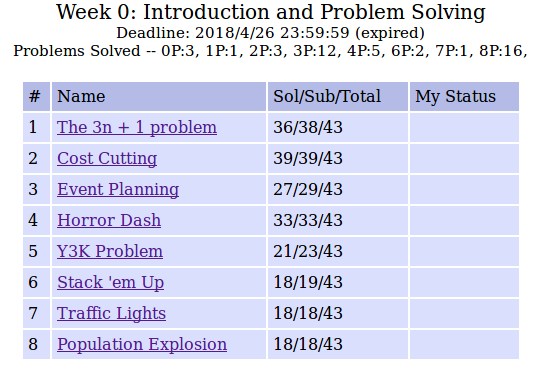
\includegraphics[width=0.8\textwidth]{img/resultW0}
    
    \bigskip

    Hope you enjoyed the warm up!
  \end{center}

\end{frame}

\begin{frame}[fragile]
  \frametitle{Comments from e-mails and questions -- 1}

  \begin{block}{Submission with Java}
    Two students had \structure{``runtime error''} with Java last week
    -- don't forget that your start class MUST be called {\bf Main}.
  \end{block}

  \vfill

\begin{verbatim}
class Main {
  public static void main(String[] args) {

    // do something...

  }
}
\end{verbatim}
\end{frame}

\begin{frame}
  \frametitle{Comments from e-mails and questions -- 2}
  \begin{block}{Input/Output}
    Two other students had problems because their program printed ``Please enter a number''.

    \bigskip

    You are very kind, but please {\bf follow the specifications} strictly!
  \end{block}
  
  \vfill

  \begin{block}{Format for MANABA submission}
    One student asked if the code for MANABA had to be the same as the code for UVA.

    \bigskip

    Yes. The code you submit on MANABA must be {\bf exactly the same}
    as the code you submitted for UVA.
  \end{block}
\end{frame}

\begin{frame}
  \frametitle{Short comments about the problems:}
  \begin{itemize}
  \item Cost Cutting, Event Planning, Horror Dash -- Easiest problems (find mean, find min, find min);
    \bigskip

  \item 3n+1 -- Still easy, but a few traps -- example of {\bf Memoization};
    \bigskip

  \item Y3K Problem -- Still easy, but skip year can be a bit troublesome.
    
  \end{itemize}
\end{frame}

%\begin{frame}
%  \frametitle{Comments about the problems}
%\end{frame}


\subsection{Outline}

\begin{frame}
  \frametitle{Quick Review of Last Week}
  \begin{itemize}
  \item \structure{Linear Arrays} (unidimensional and bidimensional) are 
    KISS data structures;
    \begin{itemize}
    \item A lot of problems can be solved by iterating on arrays
    \item Always allocate a bit more than you need.
    \end{itemize}

    \medskip

  \item \structure{Bitmasks} are quick and efficient ways to store sets of
    True/False values;

    \medskip
    
  \item \structure{Tree data structures} can search very efficiently
    \begin{itemize}
    \item Instead of implementing your own, learn to use the
      structures available from the library.
    \end{itemize}
  \end{itemize}
\end{frame}

\section{Search}

\subsection{Definitions}
\begin{frame}
  \frametitle{Topic for this week: Search}

  \begin{block}{What is Search}
    In day to day life, we say we are \structure{searching} for
    something when we are trying to find where this something is
    located.

    \begin{itemize}
    \item Keys of your bycicle;
    \item Your wallet;
    \item Your cellphone;
    \end{itemize}

    When searching, we think of our \structure{Goal} (the thing we are
    searching), and the \structure{search space} (the number of places
    where the thing could be hidden)
    
  \end{block}
  
  {\smaller
  \hfill \emph{The thing you search is always in the last place you look}\\
  \hfill (\emph{By definition!})}
\end{frame}

\begin{frame}
  \frametitle{What is a ``Search Problem''?}
  {\small
    
    We call a problem a search problem, if we can describe the problem
    as checking multiple \emph{answers} in order to find one or more
    \emph{solutions}.

    \medskip

    \begin{itemize}
    \item Answers to a search problem could be \structure{correct} or \alert{incorrect};
    \item Answers can also possibly have higher or lower \structure{scores};
    \item We can \structure{sort} the answers by score, or by some other criteria;
    \end{itemize}

    \bigskip

    Many problems in programming challenges can be described as search
    problems! (even if sometimes there are better ways to describe
    them)
  }
\end{frame}

\begin{frame}
  \frametitle{Sample Search Problems}
  \begin{block}{Traffic Lights (Week 0)}  
    You are given a set of traffic lights with different \emph{period lengths}
    \alert{Find} The moment in time when all trafic lights are in the
    green period.

    \bigskip

    \structure{Search Space:} The point in time from 1 to MCM(traffic lights).
  \end{block}

  \begin{block}{File Fragmentation (Week 2)}
    You are given a set of binary fragments. \alert{Find} a binary
    value that match all existing fragments.

    \bigskip

    \structure{Search Space:} The set of all binary values with size $< n$
  \end{block}

\end{frame}


\begin{frame}
  \frametitle{Now you are thinking with search spaces}

  When we define a problem as a search problem, we can use strategies
  based on organizing the search space, and systematically examining
  each solution contained in it.

  \bigskip

  Questions about the algorithm:
  \begin{itemize}
  \item How is the search space represented?
  \item How are the solutions ordered?
  \item In what order are the solutions tested?
  \item How many solutions are tested?
  \end{itemize}
\end{frame}

\begin{frame}
  \frametitle{Thinking with search spaces: File Fragmentation}
  \begin{itemize}
  \item \structure{How is the search space represented?}\\
    For each possible solution $n$, the binary representation of $n$ is stored.
  \item \structure{How are the solutions ordered?}\\
    The solutions are ordered by the number of fragments that do not match $n$;
  \item \structure{In what order are the solutions tested?}\\
    We can test the solutions in increasing order;
  \item \structure{How many solutions are tested?}\\
    Any item that matches all fragments is returned.
  \end{itemize}  

  \bigskip

  Of course, for many problems there is more than one way to fill this
  pattern.
\end{frame}

\begin{frame}
  \frametitle{Search Paradigms}
  These are some common approaches for search problems:
  
  \begin{itemize}
    \item Complete Search/Brute Force;
    \item Divide and Conquer;
    \item Greedy Approach;
    \item Dynamic Programming (Next week!)
  \end{itemize}

  \bigskip

  As we said before, some problems can use multiple approaches (but
  not all of them are equally good!)
\end{frame}

\subsection{Examples}

\begin{frame}
  \frametitle{Theoretical Example (1)}

  \begin{block}{Search Space}
    You have an array $A$ of $n$ integers ($n < 10K$), where the value
    of each integer $a_i$ is ($0 \leq a_i \leq 100K$).
  \end{block}
  
  \bigskip

  Imagine the following problems:
  \begin{itemize}
  \item Find the Largest and the smallest element of $A$;
  \item Find the $k^{th}$ smallest element of $A$;
  \item Find the largest gap $G$ such that $x,y \in A$ and $G = |x-y|$;
  \item Find the longest increasing subsequence of A;
  \end{itemize}
\end{frame}

\begin{frame}
  \frametitle{Theoretical Example (2)} 

  {\smaller
  How costly would be to search the solutions for each of the four
  problems described?

  \bigskip
  
  \begin{itemize}
  \item Find the Largest and smallest element of $A$: O(n) - single
    pass, and we cannot really go faster than this.
  \item Find the $k^{th}$ smallest elements of $A$:
    \begin{itemize}
    \item Repeat the search k times: $O(n^2)$ in the worst case;
    \item Order the number and search: $O(n\text{log}n)$
    \end{itemize}
  \item Fing the largest gap:
    \begin{itemize}
    \item Try all possible pairs: $O(n^2)$
    \item Greedy: Find the smallest and largest numbers $O(n)$ (you
      have to prove this works)
    \end{itemize}
  \item Longest increasing subsequence:
    \begin{itemize}
    \item Test all possible subsequences (brute force): $O(2^n)$
    \item Dynamic programming: $O(n^2)$
    \item Greedy search: $O(n\text{log}k)$ -- can you prove this?
    \end{itemize}
  \end{itemize}  
  }
\end{frame}

\section{Complete Search}
\subsection{Definition}
\begin{frame}
  \frametitle{Complete Search/Brute Force (1)}

  \structure{Complete Search} algorithms are expected to test all (or
  almost all) solutions.

  \bigskip

  \begin{exampleblock}{}
  Complete Search are usually called ``Brute Force''. But because they
  are often the best way to solve a problem, we use a nicer name here.
  \end{exampleblock}
\end{frame}


\begin{frame}
  \frametitle{Complete Search/Brute Force (2)}

  Structure of a Complete Search:

  \bigskip

  \begin{itemize}
  \item Test all existing solutions\\
    Usually achieved through either for loops or recursive calls;

    \bigskip

  \item Prune, Prune, Prune\\
    Remove bad solutions (or bad sets of solutions) as you go, by 
    ``breaking'' early form loops, or setting good ending conditions 
    to the recursive calls.
  \end{itemize}
  
\end{frame}

\subsection{True Example 1}
\begin{frame}
  \frametitle{Complete Search Example: UVA 725 -- Division}
  \begin{block}{Problem Summary}
    Given an integer N, find all pairs of numbers $abcde$ and $fghij$ so that 
    $fghij/abcde = N$ and all 10 digits are different.

    \bigskip

    \structure{Example:} $N = 62$

    \medskip

    79546 / 01283 = 62\\
    94736 / 01528 = 62\\
  \end{block}

  \vfill
  
  Consider this problem for a bit before I show how to solve it using search.
\end{frame}

\begin{frame}[fragile]
  \frametitle{Complete Search Example: UVA 725 -- Division}
  {\smaller
  \begin{block}{Full Search Solution:}
    A naive way to solve the problem is to test all $0 \leq x \leq
    99999$, calculate $y = x*n$, and test whether $x$ and $y$ have 
    all different digits.
  \end{block}

\begin{verbatim}
for (int x = 0; x < 99999; x++)
{
  y = x*n;
  digits = test(x,y);
  if (digits == 1<<10 - 1) printf("%0.5d/%0.5d=%d\n",y,x,N);
}

int digits(int x, int y)
{
  int used = (x < 10000);
  int tmp; 
  tmp = x; while (tmp) {used |= 1 << (tmp%10); tmp /= 10; }
  tmp = y; while (tmp) {used |= 1 << (tmp%10); tmp /= 10; }
  return used;
}
\end{verbatim}
  
  }
\end{frame}

\begin{frame}
  \frametitle{Complete Search Example: UVA 725 -- Division}
  Pruning the complete loop:

  \bigskip

  \begin{itemize}
  \item What is the absolute minimum and maximum for x? 01234:98765

    \bigskip

  \item Maximum for Y is also 98765, so the actual maximum for x is 
    $x < 98766/n$

    \bigskip

  \item Can we cut the digits test earlier?
  \end{itemize}
\end{frame}

\subsection{Considerations}

\begin{frame}
  \frametitle{Considerations about complete search}
  \begin{itemize}
  \item A bug-free complete search should ALWAYS be correct.\\
    \begin{itemize}
    \item A complete search tests all solutions, so it should always
      find the correct one;
    \item Of course, in many cases, checking all solutions takes too long;
    \end{itemize}

    \bigskip

  \item Complete Search should always be solution considered (KISS
    principle)
    \begin{itemize}
    \item If the problem is so small that a better solution is overkill;
    \item If you are running out of ideas, or take too many WAs;
    \item Prune, prune, prune!
    \end{itemize}
    
    \bigskip

  \item Sometimes, you can use a simple complete search on a hard
    problem to get an idea of what sort of result is expected.
    \begin{itemize}
    \item Use it to generate solutions for test cases in problems that
      generate TLEs.
    \end{itemize}
  \end{itemize}
\end{frame}

\subsection{Example 2}

\begin{frame}
  \frametitle{Complete Search Example 2: Simple Equations}
  \begin{block}{Problem Summary -- UVA 11565}
    Find $x,y,z$ so that $x+y+z=A$, $x*y*z=B$, $x^2+y^2+C^2=C$, $1
    \leq A,B,C \leq 10000$.

    \bigskip
  \end{block}

  \vfill

  We need to test sets of x,y,z, but how do we set the limits for
  these values?
\end{frame}

% First take x^2+y^2+z^2 = C. Since maximum C is 10000, and X,Y,Z must be 
% different, the maximum range of x is -100 to 100. The Reasoning goes for 
% Y and Z. With this we can do a triple loop with about 8M operations.

\begin{frame}[fragile]
  \frametitle{Example 2: Simple Equations -- initial pruning}

  \begin{block}{}
    Consider $x^2 + y^2 + x^2 = C$. Since $C \leq 10000$, the maximum
    range for $x,y,z$ must be $-100, 100$.
    
    \bigskip

    Therefore, here is the \structure{Complete Search Loop}    
  \end{block}

{\smaller
\begin{verbatim}
bool sol = false; int x,y,z;
for (x = -100; x <= 100 && !sol; x++)
  for (y = -100; y <= 100 && !sol; y++)
    for (z = -100; z <= 100 && !sol; z++)
      if (y != x && z != x && z != y &&
          x + y + z == A && x * y * z == B && x*x + y*y + z*z == C) {
             if (!sol) printf("%d %d %d\n", x,y,z);
             sol = true;
          }
\end{verbatim}

\begin{block}{}
  Can you think of other ways to prune the loop?

  
\end{block}
}
\end{frame}

\begin{frame}
  \frametitle{Example 2: Simple Equations -- more pruning}
  There are many other ways that we can prune the loop:

  \medskip

  \begin{itemize}
  \item We can change the range using the actual input values of $A,B,C$
  \item We only need one solution. We can break the loop once we find it.
  \item We can consider the other two equations, specially equation 2.
  \end{itemize}

  \vfill

  \begin{alertblock}{}
    This week's problem: ``Simple Equations -- Extreme!'' has a much
    higher range for $A,B,C$. You need a lot of pruning to avoid a TLE!
  \end{alertblock}
\end{frame}

\subsection{Complete search: TIPS}

\begin{frame}
  \frametitle{Complete Search: TIPS 1}
  The biggest issue with ``Complete Search'' solutions is: Will it
  pass the time limit? 

  \medskip

  If you think that your program is borderline passable, it might be
  worth it finding and optimizing the critical part of the code.

  \vfill

  {\smaller
  \begin{block}{Tip 1 -- Filtering Vs Generating}
    \structure{Filter Programs} examine all solutions and remove
    incorrect ones. Generally iteractive. Generally easier to
    code. Example: Request for proposal.

    \bigskip

    \structure{Generating Programs} gradually build solutions and
    prune invalid partial solutions. Generally recursive. Generally
    faster. Example: 8 queens.
  \end{block}}
\end{frame}

\begin{frame}
  \frametitle{Complete Search: TIPS 2}
  {\smaller
    \begin{block}{Tip 2 -- Prune Early}
      In the N queen problem, if we imagine a recursive solution that
      places 1 queen per column, we can prune rows, columns and
      \structure{DIAGONALS}. 

      \smallskip

      Also remember to mark impossible places when you enter the
      recursion, and unmark when you leave, using bitmasks.
      %%% 2.A - Finding simmetries can help, but it is often not worth the troube.
    \end{block}

    \vfill

    \begin{block}{Tip 3 -- Pre-computation}
      Sometimes it is possible to generate tables of partial solutions. 

      \medskip

      Load this data in your code to accelerate computation (at the
      expense of memory). The programming cost is high, since you have
      to output the tables in a way to facilitate putting it in the
      code.
    \end{block}

    }
\end{frame}


\begin{frame}
  \frametitle{Complete Search: TIPS 3}
  {\smaller
    \begin{block}{Tip 4 -- Solve the problem backwards}
      Sometimes a less obvious angle of attack may be easier.

      \medskip

      Example: UVA 10360, Rat Attack. A 1024 x 1024 city has $n \leq 20000$ rats in
      some of its blocks. You have a bomb with radius $d \leq
      50$. Where do you place the bomb to kill most rats?

      \medskip

      \structure{Obvious Approach}: Check each of the $1024^2$
      cells. Cost: $1024^2*50^2 = 2621M$ TLE

      \medskip

      \structure{Backwards Approach}: Make a 1024x1024 matrix of
      ``killed rats''. For each rat group, add its value to each cell in the 
      bomb radius: $n * d^2 = 20000*2500 = 50M + 1024*1024$.
    \end{block}
    
  }
\end{frame}

\begin{frame}
  \frametitle{Complete Search: TIPS 4}

  {\smaller
    \begin{block}{Tip 5 -- Optimizing the source code}
      \begin{itemize}
      \item Loops are usually faster than recursion
      \item Using built-in data types is usually faster than arrays/vectors
      \item Printf is usually faster than CIN/COUT
      \item Many other tips

        \bigskip
        
      \item Don't forget the Time Optimization vs. Programmer
        Optimization tradoff!
      \end{itemize}
      
    \end{block}
  }
\end{frame}

%%%% 3.3 Divide and conquer

\section{D\&C}
\subsection{Divide and Conquer}
\begin{frame}
  \frametitle{Divide and Conquer}



  Divide and Conquer (D\&C) is a problem-solving paradigm in which a
  problem is made simpler by 'dividing' it into smaller parts.

  \begin{itemize}
  \item Divide the original problem into sub-problems;
  \item Find (sub)-solutions for each sub-problems;
  \item Combine sub-solutions to get a complete solution;
  \end{itemize}

  \begin{block}{Examples}
    Quick Sort, Binary Search, etc...
  \end{block}
\end{frame}

\begin{frame}
  \frametitle{Canonical Divide and Conquer}
  \begin{enumerate}
  \item Sort an static array;
  \item You want to find item $n$.
  \item Test the middle of the array.
  \item If $n$ is smaller/bigger than the middle, throw away the second/first half.
  \item Repeat
  \end{enumerate}
  
  \vfill

  Search time: O(log n) plus sorting time if necessary.
\end{frame}

%\begin{frame}
%  \frametitle{Binary Search on Uncommon Data St
%\end{frame}

%%% Binary Search on Uncommon Data Structures
%% Example: Parents in a tree: Find the parent of node V that has value over P
% which is closest to the root. Q <= 20K, N <= 80K
%% Naive approach: For each note, search all parents. Worst case is QN (TLE)
%% Divide and conquer approach: Take each path from the root, and solve all
% Queries for each root, using binary search == O(QlogN)

\begin{frame}
  \frametitle{Binary Search on open ended problems -- Bisection}
  \begin{block}{Problem Example: Paying the debt}
    You have to pay $V$ dollars. You pay $D$ dollars per month, in $M$
    months. Each month, before paying, your debt increases by $i$. 

    \medskip

    If we fix $M$,$I$ and $V$, what is the minimal $D$?
  \end{block}

  Bisection approach:
  \begin{itemize}
  \item Estimate a good min,max interval for $D$.
  \item Select the middle value and simulate the result.
  \item If the result is bigger/smaller than the desired, modify the
    interval accordingly.
  \item Repeat.
  \end{itemize}
\end{frame}

\begin{frame}
  \frametitle{Bisection Method -- Example}
{\smaller
\begin{block}{}
$m = 2, v = 1000, i = 0.1, d = 576.19$

\medskip

After one Month, debt = 1000 x 1.1 - 576.19 = 523.81\\
After two Months, debt = 523.81 x 1.1 - 576.19 = 0
\end{block}

Bisection method: Choose the range [a..b], (ex: 0.01 1100.00)\\
Do a binary search for d in this range
}

\medskip

{\tiny
\begin{tabular}{c|c|c|c|l}
 a & b & d & simulation: f(d,m,v,i) & action: \\
 \hline
 0.01 & 1100.00 & 550.005 & undershoot by 54.9895 & increase d\\
 550.005 & 1100.00 & 825.0025 & overshoot by 522.50525 & decrease d\\
 550.005 & 825.0025 & 687.50375 & overshoot by 233.757875 & decrease d\\
 550.005 & 687.50375 & 681.754375 & overshoot by 89.384187 & decrease d\\
 550.005 & 618.754375 & 584.379688 & overshoot by 17.197344 & decrease d\\
 550.005 & 584.379688 & 567.192344 & undershoot by 18.896078 & increase d\\
 567.192344 & 584.379688 & 575.786016 & undershoot by 0.849366 & increase d\\
 ... & ... & ... & a few iterations later ... & ...\\
 ... & ... & 576.190476 & stop; error is now less than e & answer = 576.19\\
\end{tabular}
}

\medskip

{\smaller
Total number of iterations is $O(log_2((b-a)/e))$\\
UVA - 11936 - Through the desert - uses this logic}
\end{frame}

%%%% 3.4 Greedy 
\section{Greedy}
\subsection{Greedy}
\begin{frame}
  \frametitle{Greedy}

  \begin{block}{Definition}
    An algorithm is said to be greedy if it makes the locally optimal
    choice at each step, with the hope of eventually reaching the
    global optimal.
  \end{block}

  \vfill

  For greedy to work, a problem must show two properties:
  \begin{enumerate}
  \item It has optimal sub-structures (Optimal solution of the problem
    contains optimal solutions for the sub-problems)
  \item It has the greedy property: Making locally optimal choices
    will lead ``eventually'' to the optimal solution (difficult to
    prove!)
  \end{enumerate}

\end{frame}

\begin{frame}
  \frametitle{Greedy Example 1 -- Coin Change}

  Given a target value $V$ and a list of coin sizes $S$, what is the
  minimum number of coins that we must use to represent $V$?

  \bigskip

  \begin{block}{Example:}
    $V = 42, Coins = 25, 10, 5, 1$\\
    {\small (a 1\$ coin means we can always make any value)}
  \end{block}

  \bigskip

  We can solve this case by always taking the biggest coing that fits
  the remaining cost: 25x1, 10x1, 5x1, 1x2;

  \medskip

  However, if V = 6, and coins = 4,3,1, this greedy algorithm does not
  reach an optimal solution.

  \begin{center}
    Be careful that \alert{a greedy algorithm can be wrong!}
  \end{center}
\end{frame}

\begin{frame}
  \frametitle{Greedy Example 2 -- Load Balancing UVA 410}

  \begin{block}{Problem Description}
    

  You have C chambers, and S < 2C specimens with different positive
  weights. You need to decide where each specimen should go to
  minimize ``imbalance''.
  \end{block}
  
  \begin{equation*}
    \text{Imbalance} = \sum_{i=1}^C |CM_i - AM|
  \end{equation*}

  Can you figure out a greedy search solution?
\end{frame}


\begin{frame}
  \frametitle{Greedy Example 2 -- Load Balancing UVA 410}

  \begin{block}{Problem Description}
  You have C chambers, and S < 2C specimens with different positive
  weights. You need to decide where each specimen should go to
  minimize ``imbalance''.
  \end{block}

  Insights:

  \begin{itemize}
  \item A chamber with 1 individual is always better than a chamber
    with 0 individuals.

    \medskip

  \item Order of chambers does not matter.
  \end{itemize}
  %%% Make people think for a while here.
\end{frame}

\begin{frame}
  \frametitle{Greedy Example 2 -- Load Balancing UVA 410}

  \begin{block}{Problem Description}
  You have C chambers, and S < 2C specimens with different positive
  weights. You need to decide where each specimen should go to
  minimize ``imbalance''.
  \end{block}

  \vfill

  \structure{Greedy algorithm:} Order the individuals by weight, and 
  put one in each chambers until the chambers are full, then add one
  in each chamber backwards.

  \bigskip

  A similar approach can be used to solve this week's problem ``Dragon
  of LooWater''.
\end{frame}

%%%%%%%%%%%%%%%%%%%%%%%%%%%%%%%%%%%%%%%%%%%%%%%%%%%%%%%%%%%%%%%%%%%%%%%%%%%%%%%%%%%%%%%%
%%% State Space Search
% UVA 11212 Editing a Book
% You can cut pages (in order) and paste them to correct the order of the book
% Report number of steps required.
% Upper bound: k-1 (paragraphs in the wrong position) - not correct answer, examples
% Calculations on the number of states for the problem (No solution given in the slides)



\section{Week's Problems}
\subsection{Problem Discussion}

\begin{frame}
  \frametitle{This Week's Problems}
  \begin{itemize}
  \item Dominator
  \item Forwarding Emails
  \item Ordering
  \item Place the Guards
  \item Doves and Bombs
  \item Come and Go
  \item ACM Contest and Blackout
  \item Ancient Messages
  \end{itemize}
\end{frame}

\begin{frame}
  \frametitle{Problem Hints (0)}

  {\smaller
  \begin{block}{Library!}
    For many of these problems, you will use a lot of repeated code:
    \begin{itemize}
    \item Visited Node arrays;
    \item Adjacent lists;
    \item Parent nodes;
    \end{itemize}

    \bigskip

    Prepare a template for the most common codes you use, and
    copy-paste it whenever necessary!
  \end{block}
  \begin{block}{Tricky Cases}
    \begin{itemize}
    \item Graphs with 1 or 0 Vertex
    \item Unconnected Graphs
    \item Self Loops
    \item Double edges
    \end{itemize}
  \end{block}
  }
\end{frame}

\begin{frame}
  \frametitle{Problem Hints (1)}  
  {\smaller
    \begin{block}{Dominator}
      \begin{itemize}
        \item If All paths from 0 to node B pass through node A, then node A {\bf dominates} node B;
        \item For all pair of nodes $i,j$, output ``Y'' if $i$ {\bf dominates} $j$, or ``N'' if not;
      \end{itemize}
    \end{block}

    \bigskip

    The idea of this problem is one of ``reachability'' -- can I reach
    node $j$ if I remove node $i$ from the graph?

    \bigskip

    Note: if $j$ is not connected to ``0'', then \emph{no one dominates j}
  }
\end{frame}

\begin{frame}
  \frametitle{Problem Hints (2)}
  {\smaller
    \begin{block}{Forwarding Emails}
      Every person $i$ sends e-mail only to person $j$.
      
      \bigskip
      
      What is the longest email chain?
      
      \bigskip
      
      Where does it start?
    \end{block}
    
    \begin{itemize}
    \item How do you deal with loops?
    \item Time limit is not very large, Try to find an O(n) solution!
    \end{itemize} 
  }
\end{frame}

\begin{frame}
  \frametitle{Problem Hints (3)}
  {\smaller
    \begin{block}{Ordering}
      Print all possible Orderings of a Direct Acyclic Graph

      \bigskip

      Generalize the DAG ordering algorithm which we discussed in class.
    \end{block}
    
    \begin{block}{Palace Guards}
      \begin{itemize}
        \item How do you represent the roads and junctions as a Graph?
        \item Find a ``guard-no guard'' assignment to vertices of the
          graph.
        \item First test if a solution is possible!
      \end{itemize}
    \end{block}    
  }
\end{frame}

\begin{frame}
  \frametitle{Problem Hints (4)}
  {\smaller
    \begin{block}{Doves and Bombs}
      This problem is about finding ``critical vertices'' in a
      graph. But how do you calculate the ``pigeon value'' of a
      vertex?
    \end{block}

    \begin{block}{Come and Go}
      Straight implementation of ``Strong Connected Components''. Be
      careful with tricky graphs!
    \end{block}    
  }
\end{frame}

\begin{frame}
  \frametitle{Problem Hints (5)}
  {\smaller
    \begin{block}{ACM Contest and Blackout}
      Goal: Find the {\bf First} minimum spanning Tree and the {\bf
        Second} minimum spanning Tree
    \end{block}

    \bigskip
    
    \begin{itemize}
    \item In this class we discussed how to find the Minimum Spanning Tree      
    \item How would we find the {\bf second minimum?}
    \item Idea: Maybe if we remove some edges from the graph?
    \end{itemize}
  }
\end{frame}

\begin{frame}
  \frametitle{Problem Hints (6)}
  \begin{block}{Ancient Message -- Challenge problem!}
    Count the symbols inside an image -- order does not matter!

    \bigskip

    What is the {\bf Main} difference between the symbols?
  \end{block}
    
  \begin{itemize}
  \item The shape and size of the symbols is actually not important!
  \item Before you begin programming, discover what is the real
    difference between the symbols.
  \item Hint: The numbers ``1'', ``0'', ``8'' have the same difference.
  \end{itemize}    
\end{frame}



\section{Extra}
\subsection{Search Research}
%% TODO: Improve the Search Algorithms in CS research ... Next time!

\begin{frame}
  \frametitle{Search Algorithms in CS Research}

  Complete Search and Greedy algorithms feel like something that you
  only use in your first year of Computer Science, and then never
  touch again..

  \vfill

  ... it turns out however, that search algorithms have a really
  important role: Heuristics and NP-hard problems.
\end{frame}

\begin{frame}
  \frametitle{Heuristic Example: A* Search} 

  A* is a search algorithm for finding a shortest path between two
  (x/y) coordinates.

  {\small
  \begin{enumerate}
  \item List all vertices that you can check next;
  \item Sort the vertices by sum(distance from start + distance from goal)
  \item Explore vertice highest in the sort;
  \end{enumerate}
  }

  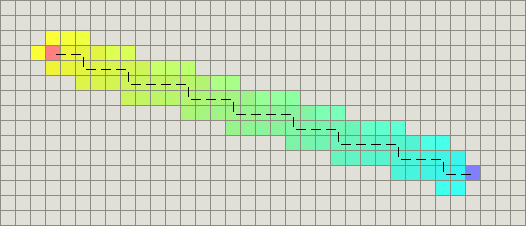
\includegraphics[width=0.4\textwidth]{../img/astar2_amitpatel}\hfill
  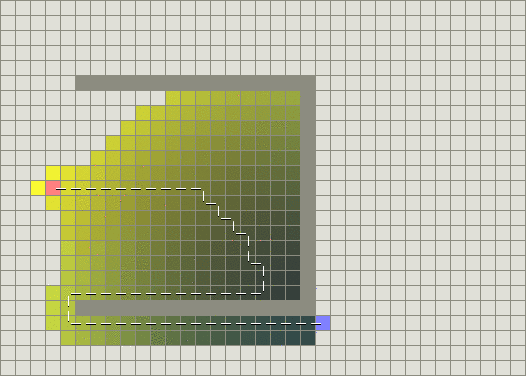
\includegraphics[width=0.4\textwidth]{../img/astar_amitpatel}

  \hfill{\tiny Images from Amit Patel}

\end{frame}

\begin{frame}
  \frametitle{Heuristic and NP-hard problems}

  Consider NP-hard problems:
  \begin{itemize}
  \item There are no polinomial algorithms that solve the problem;
  \item However, a solution to the problem can be \structure{tested}
    in polinomial time;
  \end{itemize}

  \bigskip

  One approach to NP-hard problems is to treat them as
  \structure{search problems}, systematically testing solutions 
  (in polynomial time), until an acceptable solution is found.
\end{frame}

\begin{frame}
  \frametitle{Heuristic Algorithms}
  \begin{itemize}
  \item Hill Climbing
  \item Evolutionary Algorithms
  \item Swarm Algorithms
  \item Etc...
  \end{itemize}
\end{frame}

\begin{frame}
  \frametitle{Next Week}
  \begin{center}
    Dynamic Programming!
  \end{center}
\end{frame}

\end{document}
